\chapter{Úvod}
V následující části práce navážeme na předchozí obecnou část a zaměříme se na dva zbylé cíle, které jsme definovali v úvodu.\par
\paragraph{Jsou jimi:}
\begin{itemize}
    \item Navrhnout systém pro vyhledávání osob a pracovišť dle kompetencí a provést rešerši dostupných dat
    \item Implementovat prototyp systému pro vyhledávání osob a pracovišť dle kompetencí pro FEL ČVUT 
    % \item Analýza datových zdrojů osob, pracovišť a znalostí 
    % % (FEL, světové)
    % \item Popis návrhu systému pro vyhledávání osob a pracovišť dle jejich kompetencí
    % \item Popis implementace a testování prototypu řešení
\end{itemize}
Nejdříve shrneme aktuální situaci týkající se strukturalizace a kategorizace znalostí a informací na FEL ČVUT. Na to navážeme analýzou datových zdrojů. Dále rozebereme návrh systému a v poslední fázi rozebereme implementaci prototypu za použití zvolené technologie, testování tohoto prototypu a další implementační detaily.

\section{Informační infrastruktura Fakulty elektrotechnické ČVUT}
České vysoké učení technické v Praze se skládá z osmi fakult a dalších přidružených pracovišť. Jednotlivé fakulty se skládají z dalších podřazených jednotek - kateder, center a podobně.\par
Informační infrastruktura ČVUT je tvořena od katederních systémů přes fakultní až k těm univerzitním. Komunikace mezi systémy probíhá typicky jen směrem dolů (tedy od systémů výše putují data k systémům níže). Takový způsob integrace je pro toto uspořádání poměrně vyhovující.\par
\begin{figure}[htbp!]
	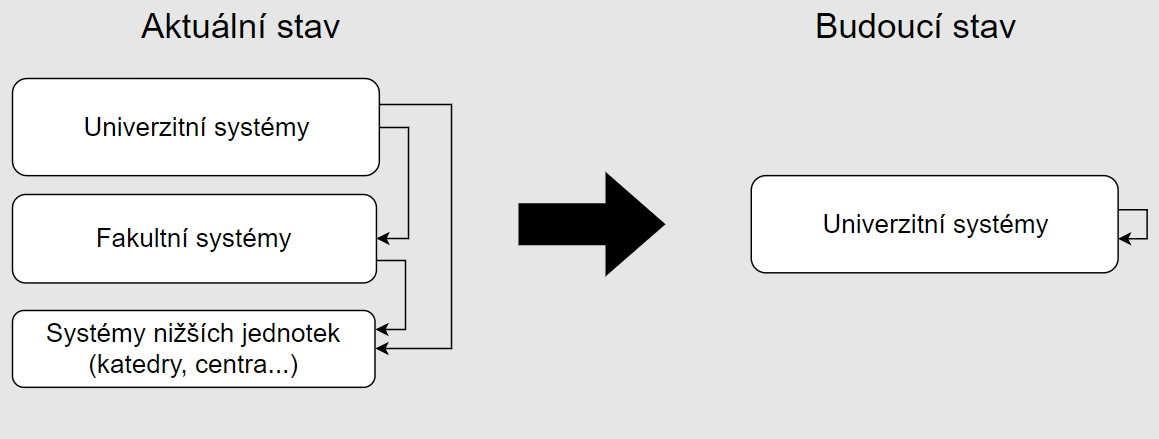
\includegraphics[width=\linewidth]{img/ctu-infrastructure.png}
	\caption{Schematické zobrazení informační infrastruktury ČVUT a komunikace systémů (zdroj autor)}
	\label{fig:ctu-infrastructure}
\end{figure}
Z dlouhodobého hlediska je tendencí strukturu zjednodušovat, tedy přesouvat kompetenci správy systémů na vyšší úrovně v hierarchii. Například tedy zamezit vzniku katederním systémům a místo toho zakládat centrální fakultní systémy. Toto řešení má výhody při změnách (ať už metodických, tak implementačních). Na druhou stranu může být toto řešení dosti personálně náročné, jelikož by se univerzita musela v budoucnu starat o všechny systémy. Zároveň by se tímto způsobem však měla spousta systémů eliminovat. Přechod na takové vnitřní uspořádání nelze provést skokově. Vhodnější jsou pozvolné změny, které však trvají velmi dlouho. \par
\noindent O jednotlivých systémech, které budou relevantní v kontextu této práce, se zmíníme v následujících kapitolách.





% a.	Úvod o fakultě, co je to za organizaci, jak zachází se znalostmi, jak je na tom informační infrastruktura.... – AS-IS
% případně navázat i TO-BE stavem - přínos pro školu